\section{Projeto Estrutural}
\subsection{Características Gerais}

O projeto estrutural se baseia na construção de um alimentador que ficará acoplado a um tanque de peixes. O alimentador guardará a ração em um armazenador que estará acoplado a um sistema de alimentação responsável por despejar na dose certa a ração para os peixes, vale ressaltar que essa dosagem deve ser feita de forma instantânea, ou seja, não pode se prolongar por períodos grandes de tempo para que os peixes menores não sejam privados de sua alimentação pelos peixes maiores.

A estrutura deverá ser robusta dado que ficará no meio do lago onde ficam os tanques de criação e está sujeito a esforços criados pelo contato com a água e vento, além de ficar exposto diretamente ao Sol. A condição de robustez se torna indispensável pois o cliente exige que a estrutura tenha capacidade de armazenamento de 300 kg, esta quantidade de ração equivale de 3 a 4 dias sem necessidade de reabastecimento.

Para a conservação das características nutricionais da ração, a estocagem correta é extremamente importante. É propício o surgimento de fungos em rações sujeitas a altas umidade e altas temperaturas, já que estarão no meio do lago, o que pode levar a perda de desempenho dos peixes, ou até a morte. Outro problema é a incidência elevada de raios solares nas rações, o que também causa prejuízo em seus componentes, fazendo também com que percam suas propriedades nutricionais. Para contornar esta situação será necessário prever um isolamento térmico eficiente.

Podemos então dividir estruturalmente o alimentador em três subsistemas: Armazenamento de ração, Sistema de Alimentação dos peixes e Suporte estrutural. Mais a frente será detalhado sobre as soluções prevista para cada subsistemas.

\subsubsection{Escolha do Material}

Levando em consideração que a estrutura deverá  flutuar sobre o lago suportando o armazenamento de 300 kg de ração e o peso próprio, decidiu-se criar uma matriz de decisões, presentes nas tabelas \ref{matriz1} e \ref{matriz2}, para que houvesse uma escolha de material mais apropriada para a confecção do alimentador. Partes da estrutura que sao submetidos a esforços diferentes, possivelmente serão confeccionados de diferentes materiais, visando a otimização do projeto e de custos. Após uma pré análise, foi levantado três possíveis materiais para a elaboração de cada subsistema estrutural. Entre os três materiais estão: chapas de aço carbono facilmente encontradas comercialmente (aço 1010), chapas de alumínio também encontradas comercialmente e a possibilidade de se trabalhar com polímeros (nylon, poliuretano ou poliacetal). Para uma análise mais simplificada e de mais fácil entendimento , ela será pontuada usamos valores de 0 a 2 sendo que o valor mais alto sempre indica uma vantagem do material. Os pontos de maior significância para a decisão do material foram: Tensão de escoamento (Sy), Preço do material, Manufatura (incluindo todos os processos de fabricação necessários), Acessibilidade, Massa do conjunto e Conservação com o efeito do tempo. Posteriormente foi atribuído um fator de multiplicação (2x) aos pontos de maior importância (Manufatura e Massa).

\begin{sidewaystable}
\begin{table}[H]
\centering
\caption{Matriz de decisão para escolha do material.}
\label{matriz1}
\begin{tabular}{|l|l|l|l|l|l|l|}
\hline
\multicolumn{1}{|c|}{Material} & \multicolumn{1}{c|}{\begin{tabular}[c]{@{}c@{}}Sy \\ (escoamento)\end{tabular}} & \multicolumn{1}{c|}{Preço} & \multicolumn{1}{c|}{Manufatura} & \multicolumn{1}{c|}{Acessibilidade} & \multicolumn{1}{c|}{Densidade} & \multicolumn{1}{c|}{Resistęncia ao tempo.} \\ \hline
Aço carbono                    & 2                                                                               & 2                          & 1                               & 1                                   & 1                              & 1                                          \\ \hline
Alumínio                       & 1                                                                               & 1                          & 2                               & 1                                   & 2                              & 2                                          \\ \hline
Polímero                       & 0                                                                               & 0                          & 0                               & 1                                   & 2                              & 1                                          \\ \hline
\end{tabular}
\end{table}

\begin{table}[H]
\centering
\caption{Matriz de decisão com pesos computados.}
\label{matriz2}
\begin{tabular}{|l|l|l|l|l|l|l|}
\hline
Material    & Sy & Preço & Manufatura (2x) & Acessibilidade & Densidade (2x) & Resistęncia ao tempo. \\ \hline
Aço carbono & 2  & 2     & 2               & 1              & 2              & 1                     \\ \hline
Alumínio    & 1  & 1     & 4               & 1              & 4              & 2                     \\ \hline
Polímero    & 0  & 1     & 0               & 1              & 4              & 1                     \\ \hline
\end{tabular}
\end{table}
\end{sidewaystable}

Após a análise das tabelas conclui-se que o alumínio tem muitas vantagens totalizando 13 pontos na matriz de decisão com pesos computados. Os materiais com menor pontuação não serão excluídos, podendo ser utilizados em diferentes partes no projeto. Apesar de ter seu uso difundido os polímeros termoplásticos em geral são utilizados principalmente para produção em larga escala, devido ao alto custo de seus moldes para injeção. Este alto custo a fabricação de peças poliméricas termoplásticas personalizadas dificulta um maior uso dos polímeros no projeto. Existe também a possibilidade de usar peças de plástico já existentes, porém seria problemático unir peças diferentes para a formação da estrutura requerida. Os plásticos poderão ser interessantes para implementação de flutuadores, além de ser vital na calafetação de peças.

As características do aço para fins estruturais sao muito boas. Porém por se tratar de uma estrutura flutuante, sua alta densidade ($7,86 \frac{g}{cm^3}$\cite{euroaktion}) comparada a do alumínio ($2,7 \frac{g}{cm^3}$\cite{euroaktion}) torna seu uso mais restrito, podendo ser utilizado como reforços na estrutura. O material também sofrerá com intempéries, podendo oxidar e assim comprometer a estrutura e ou alterar a composição da ração. Após uma análise mais detalhada da situação, foi concluído que o alumínio se adequa de forma melhor aos requisitos iniciais de projeto, tornando-o o principal material a ser utilizado na construção da estrutura.

Difundido na engenharia e de fácil acesso, o alumínio é um metal de baixa densidade, resistente, inoxidável e de fácil usinagem e manuseio. Listado abaixo estão as propriedades\cite{aluminuin} mais relevantes do alumínio comercial 1050-0, normalmente o alumínio utilizado nas chapas:

Propriedades Físicas

\begin{itemize}
  \item Densidade: $2.71 \frac{g}{cm^3}$
  \item Ponto de fusão: 650{\degree}C
  \item Expansão Térmica: $24 * 10^-6/K$
  \item Módulo de elasticidade: $71GPa$
  \item Condutividade Térmica: $222\frac{W}{m*K}$
\end{itemize}

Propriedades Mecânicas

\begin{itemize}
  \item Resistência a Tração: 65-95 MPa
  \item Tensão de escoamento: 20 MPa
  \item Dureza Brinell: 20 HB
\end{itemize}

A seguir falamos sobre cada módulo do projeto estrutural comentado nesta seção mais detalhadamente e apresentaremos as soluções pensadas pelo grupo para construção da estrutura.

\subsubsection{Armazenamento}

O armazenamento de ração é o principal problema estrutural a ser solucionado dado que a ração é o insumo mais caro e corresponde a 80\% do valor do peixe. O grande problema enfrentado pelo cliente é a falta de alimentação ao peixe nos períodos de fim de semana onde há falha por conta da mão de obra. O período em questão informado pelo cliente vai de sábado a terça-feira, e para resolver esse problema necessita-se de um armazenamento de 300 kg. Com essas questões como guias para o projeto estrutural o grupo escolheu uma solução de armazenamento que servirá como guia para os subsistemas de alimentação e suporte. A estrutura contará também com uma tampa para proteger a ração da chuva e radiação direta do Sol, além de servir como suporte para a placa solar.

Primeiramente foi necessário calcular o volume de ração que seria necessário para acumular 300 kg de ração. Uma consideração importante para esse cálculo é que o cliente usa rações de porcentagem de proteína diferentes e essas possuem densidades diferentes[3]. Além da quantidade de proteína, o tamanho da ração também varia o fator de empacotamento que faz com que as rações de dimensões maiores ocupem um volume maior para uma mesma massa. Para fazer uma primeira análise o grupo entrou em contato com um vendedor de ração que passou os valores dimensionais referentes ao saco de ração e com isso foi possível estimar o volume necessário para o armazenar essa ração e comparar com o valor encontrado na literatura, porém uma análise mais precisa desses dados será efetuada quando o cliente trazer as amostras da ração utilizada por ele. Essa reunião já está acertada e se dará no começo do mês de setembro.

\subsubsubsection{Dimensionamento do Armazenador}

Para dimensionar o armazenador utilizamos o pior caso informado pelo vendedor de ração. Vale ressaltar que o valor de densidade encontrado na literatura \cite{Omicsonline} (visto que essa informação não se encontra disponível nos sites das produtoras e revendedoras de rações) foi de $267 \frac{kg}{m^3}$ enquanto o calculado foi de $243 \frac{kg}{m^3}$. Podemos ver que os valores foram bem próximos o que ressalta a relevância dos dados, lembrando que estamos tratando do pior caso onde há a menor densidade. Abaixo estão apresentados os cálculos de densidade da ração, para o cálculo consideramos o pacote de ração como um paralelepípedo e o saco de ração possui 25 kg.

Fig Volume do paralelepípedo

Dados encontrados:

\[c = 1m\]
\[b = 0,57m\]
\[c = 0,18m\]
\[V = a.b.c = 1 . 0,57 . 0,18 = 0,1026 m^3\]
\[d = \frac{m}{v} = \frac{25}{0,1026} = 243.66 \frac{kg}{m^3}\]

Após descobrirmos a densidade da ração já levando em conta seu empacotamento, podemos dimensionar a forma do armazenador. Primeiro achamos o volume necessário para armazenar um total de 300 kg e ração, considerando uma densidade de $243.66 \frac{kg}{m^3}$ (pior caso possível).

\[V = \frac{m}{d} = \frac{300}{244} = 1,232m^3\]


Com isso sabemos que o armazenador deve possuir um volume de no mínimo $1,232m^3$ ou 1232 l. Utilizando sólidos regulares como um paralelogramo e um cilindro conseguimos descobrir os tamanhos de lado e raio respectivamente. Vamos assumir 2 casos para cada sólido.

Primeiro caso Paralelogramo- Cubo ($v=l^3$)

\[l = \sqrt[3]{1,232/2} = 1,071m\]

Segundo caso Paralelogramo- Paralelepipedo de base quadrada onde \[h = 2l ; v=l^2h\]
\[l = \sqrt[3]{1,232/2} = 0.851 m\]

Primeiro caso Cilindro -\[r = h ; v =\pi r^3\]
\[r = \sqrt[3]{\frac{1,232}{\pi}} = 0,732 m\]

Segundo caso Cilindro -\[h = 2r; v=2.\pi.r^2.h\]
\[v = 2.r^2.\pi .h = 2\pi.r^3\]
\[r = \sqrt[3]{\frac{1,232}{2\pi}} = 0,581 m\]

A partir daí temos duas geometrias diferentes com duas opções para cada. Essas opções influenciarão nas dimensões finais do alimentador e afetarão parâmetros como estabilidade, tensão suportada pelo fundo, quantidade de material utilizado, entre outros aspectos. Para um primeiro dimensionamento a primeira opção foi escolhida, um cubo de lado igual a 1,071m.

\subsubsubsection{CAD e análise de tensões}

Para uma primeira análise sobre a espessura da chapa necessária para fabricação da estrutura do armazenador foi feito um CAD prévio da geometria escolhida acima utilizando o software CATIA v5 e nele mesmo foi feita a análise em FEA (análise em elementos finitos) utilizando o ambiente de análise estrutural. Uma estrutura como base foi projetada para simular como o armazenador seria suportado no alimentador, foi projetada com base no processo de fabricação facilitado (tubos e cantoneiras) porém sua geometria ainda necessita de um projeto mais definido. Abaixo as imagens retiradas do CATIA.

\begin{figure}[H]
 \centering
   \includegraphics[keepaspectratio=true,scale=0.8]{figuras/estrutura1.eps}
 \caption{Dimensões do Armazenador}
 \label{estrutura1}
\end{figure}
\begin{figure}[H]
 \centering
   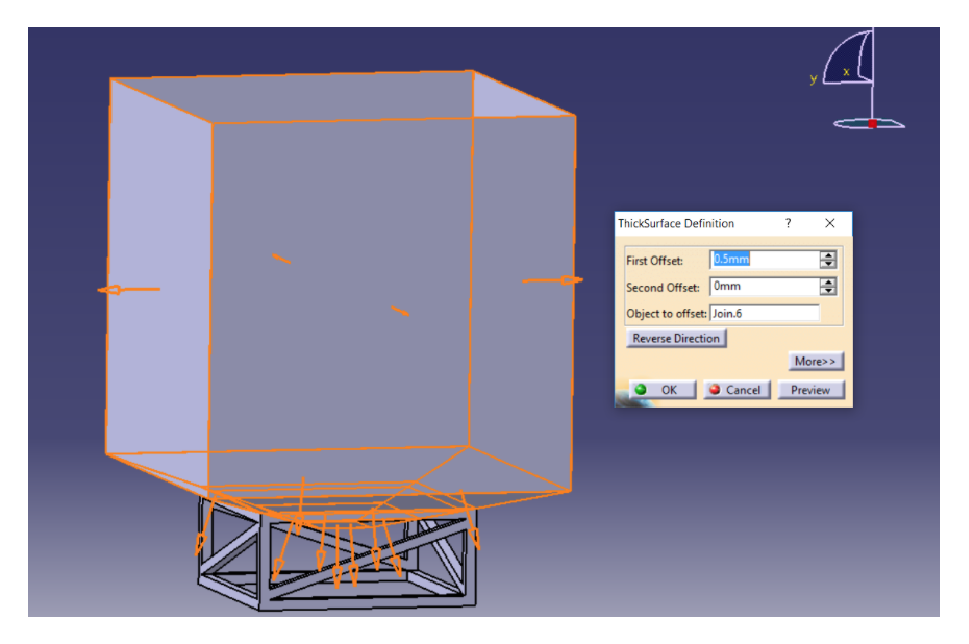
\includegraphics[keepaspectratio=true,scale=0.8]{figuras/estrutura2.eps}
 \caption{Espessura da chapa}
 \label{estrutura2}
\end{figure}
\begin{figure}[H]
 \centering
   \includegraphics[keepaspectratio=true,scale=0.8]{figuras/estrutura3.eps}
 \caption{Propriedade do material no CATIA}
 \label{estrutura3}
\end{figure}
\begin{figure}[H]
 \centering
   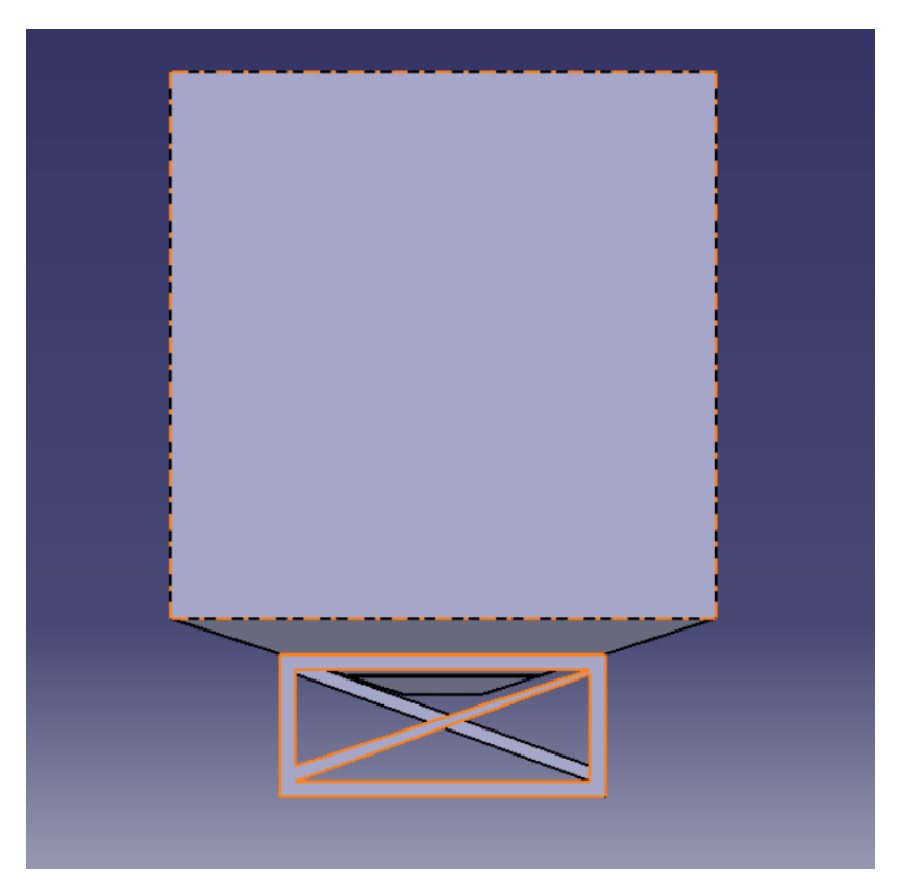
\includegraphics[keepaspectratio=true,scale=0.8]{figuras/estrutura4.eps}
 \caption{Base do Armazenador}
 \label{estrutura4}
\end{figure}

Nesta primeira análise utilizamos uma chapa de 0.5mm para forma as paredes do armazenador, lembrando que quanto menor a quantidade de material utilizado menor será a massa total da estrutura e mais barato o projeto. As dimensões de lado são as calculadas para um cubo, onde l = h = 1.072m. As propriedades do alumínio estão de acordo com as listadas anteriormente com um módulo de elasticidade (módulo de young) = $E = 71GPa = 7.10^10Pa$ onde $1Pa = 1\frac{N}{m^2}$.
Também foi construído uma tremonha, estrutura piramidal abaixo do cubo principal, que servirá para direcionar a ração para o furo por onde ela será despejada, que num primeiro momento ficará no centro da geometria. A angulação da tremonha é de 46.41º, um ângulo próximo de 45º para uma melhor distribuição da massa suportada pela estrutura e não atrapalhar o fluxo de ração.

\begin{figure}[H]
 \centering
   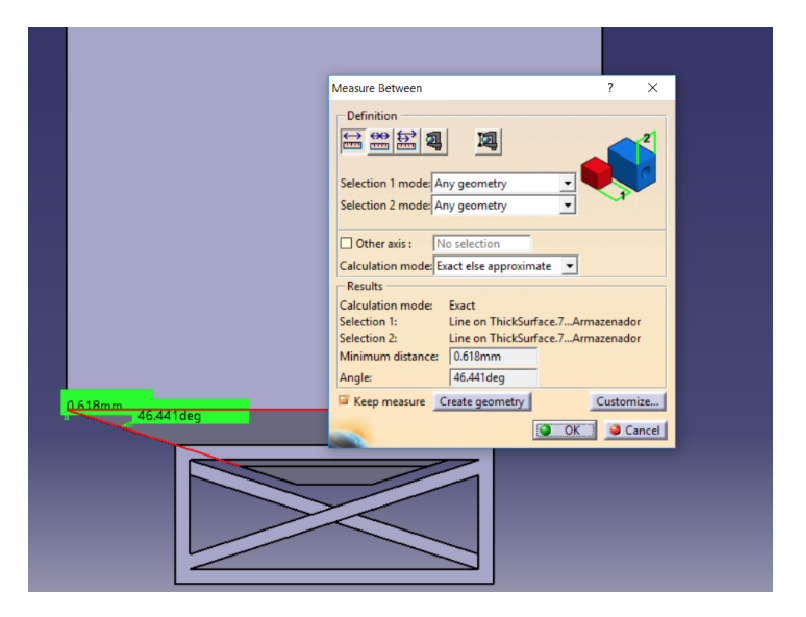
\includegraphics[keepaspectratio=true,scale=0.8]{figuras/estrutura5.eps}
 \caption{Inclinação da Tremonha}
 \label{estrutura5}
\end{figure}

Para analisar as tensões principais na estrutura foi utilizado o ambiente de análise estrutural do próprio CATIA. Essa primeira análise serve como um primeiro passo e quando as partes forem finalizadas com CADs mais precisos o grupo utilizará um software mais preciso para essa análise. O tamanho da malha foi definido em 88.95mm e a análise feita como elemento linear. Os parâmetros de análise estão detalhados abaixo

\begin{figure}[H]
 \centering
   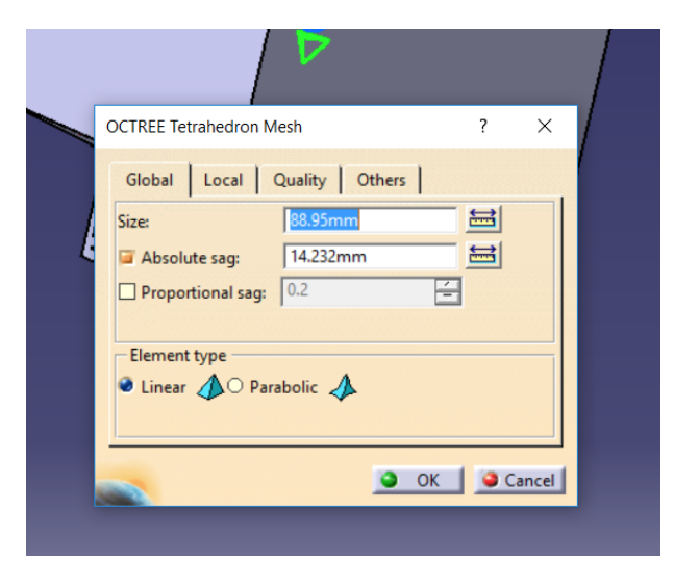
\includegraphics[keepaspectratio=true,scale=0.8]{figuras/estrutura6.eps}
 \caption{Parâmetros de análise: Global}
 \label{estrutura6}
\end{figure}
\begin{figure}[H]
 \centering
   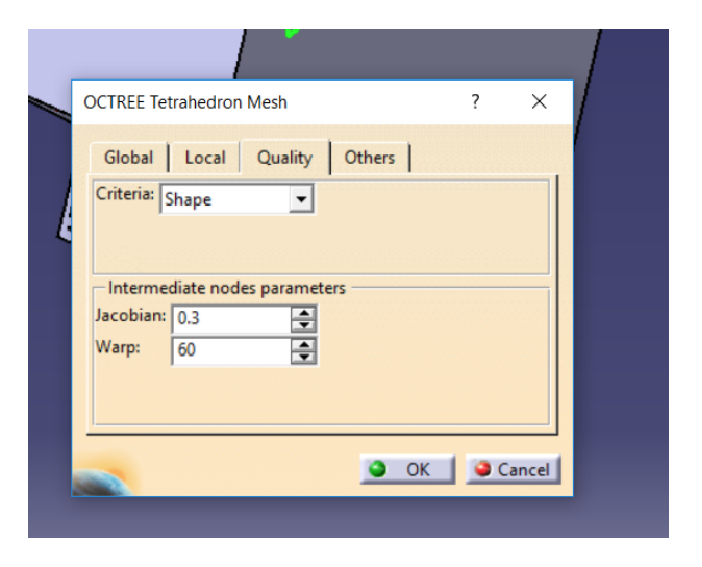
\includegraphics[keepaspectratio=true,scale=0.8]{figuras/estrutura7.eps}
 \caption{Parâmetros de análise: Qualidade}
 \label{estrutura7}
\end{figure}
\begin{figure}[H]
 \centering
   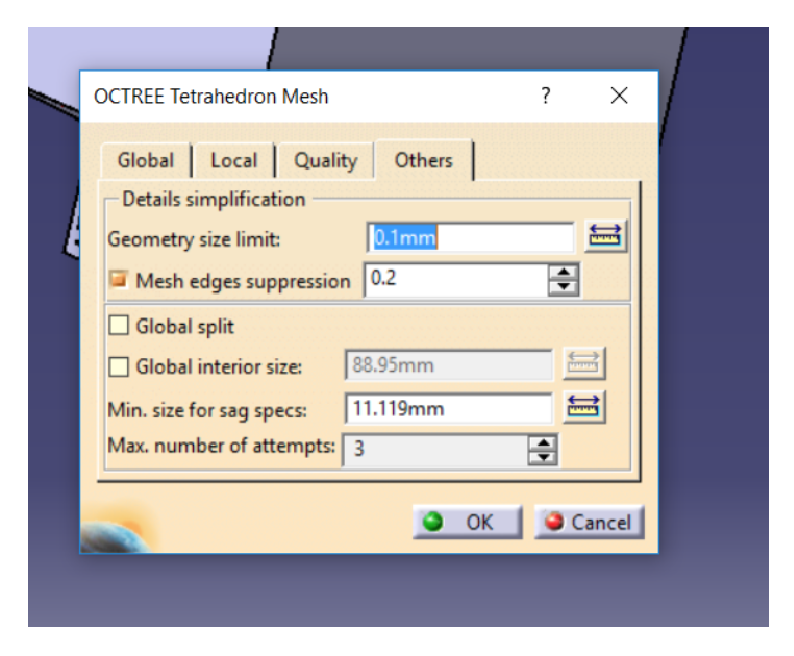
\includegraphics[keepaspectratio=true,scale=0.8]{figuras/estrutura8.eps}
 \caption{Parâmetros de análise: Outros}
 \label{estrutura8}
\end{figure}

Após esses parâmetros ajustados as restrições de movimento foram selecionadas. A estrutura foi engastada à base simulando que estaria presa ao suporte. Uma carga distribuída de 3500N foi aplicada às paredes do fundo (tremonha) simulando a carga da ração e a carga da estrutura, extrapolada. Os resultados são mostrados abaixo.

\begin{figure}[H]
 \centering
   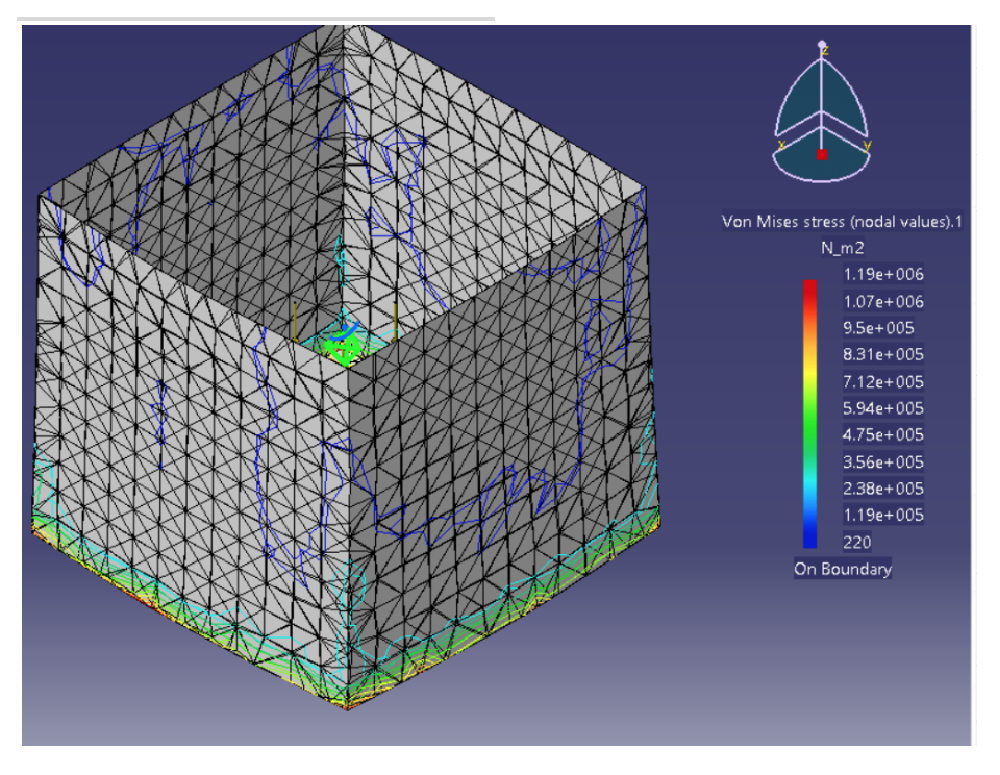
\includegraphics[keepaspectratio=true,scale=0.8]{figuras/estrutura9.eps}
 \caption{Tensão de Von Mises}
 \label{estrutura9}
\end{figure}
\begin{figure}[H]
 \centering
   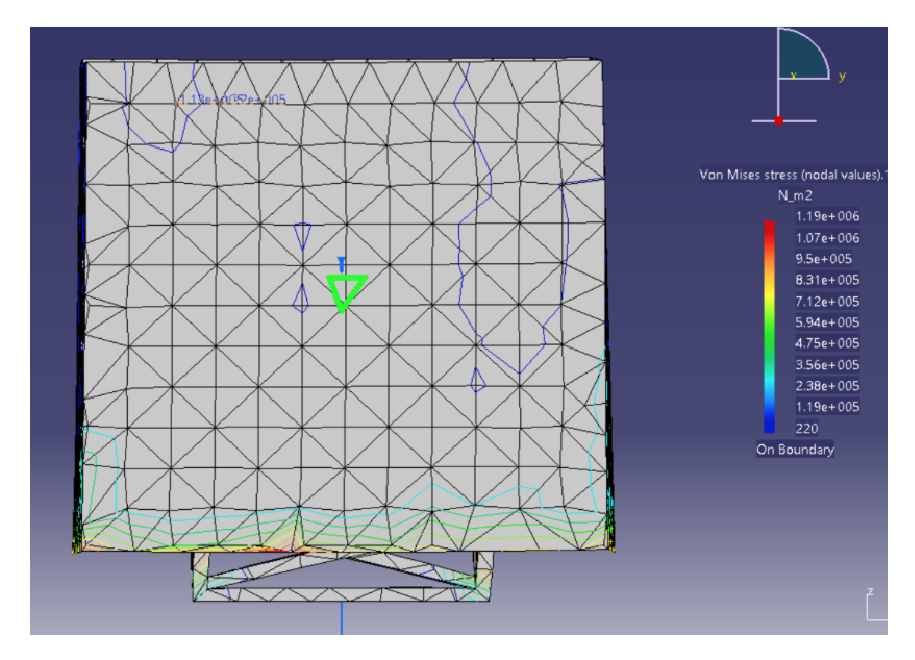
\includegraphics[keepaspectratio=true,scale=0.8]{figuras/estrutura10.eps}
 \caption{Tensão de Von Mises na base}
 \label{estrutura10}
\end{figure}

A maior tensão encontrada foi de 1.19 MPa, muito abaixo dos 20 MPa de tensão de escoamento. Então podemos verificar que mesmo com uma chapa fina de alumínio a estrutura não escoa. Porém podemos ter um problema de estabilidade devido a geometria do cubo onde a chapa pode mudar o formato devido a esforços aplicados nas paredes do cubo tendo em vista que a estrutura sofrerá ação do balanço das águas. Para resolver esse problema podemos reforçar a estrutura facilmente com cantoneiras de alumínio ou ferro chapa, aumentando um pouco o peso suportado mas com a análise de tensão percebemos que temos margem para isso.

\subsubsection{Processos de Fabricação}

\begin{figure}[H]
 \centering
   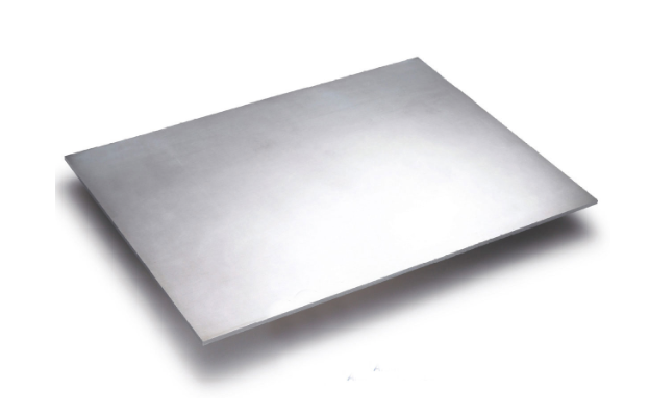
\includegraphics[keepaspectratio=true,scale=0.8]{figuras/estrutura11.eps}
 \caption{Chapa de alumínio}
 \label{chapa_aluminio}
\end{figure}

Para fabricar essa o armazenador foi pensada a utilização de chapas de alumínio comercial como a mostrada acima. Porém pesquisando o comércio local vimos que normalmente as chapas têm o comprimento de um  dos lados fixos em 1m (um metro). A ideia principal seria dobrar as chapas e formar a geometria necessária precisando fixar apenas as duas pontas. A seguir uma demonstração de como se daria a dobra pensada.

\begin{figure}[H]
 \centering
   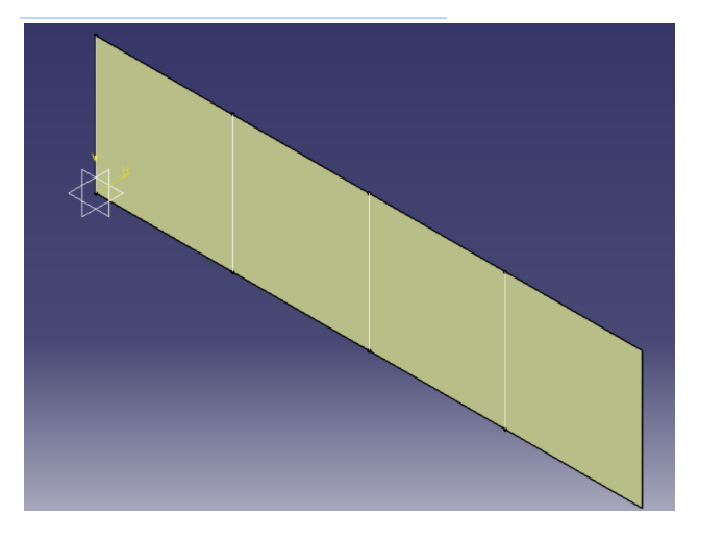
\includegraphics[keepaspectratio=true,scale=0.8]{figuras/estrutura12.eps}
 \caption{Chapa de 1m de altura}
 \label{estrutura12}
\end{figure}
\begin{figure}[H]
 \centering
   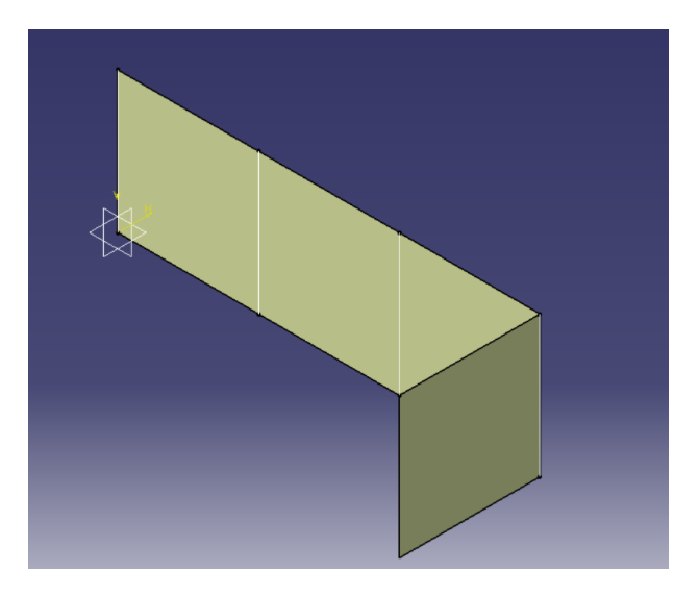
\includegraphics[keepaspectratio=true,scale=0.8]{figuras/estrutura13.eps}
 \caption{Primeira dobra}
 \label{estrutura13}
\end{figure}
\begin{figure}[H]
 \centering
   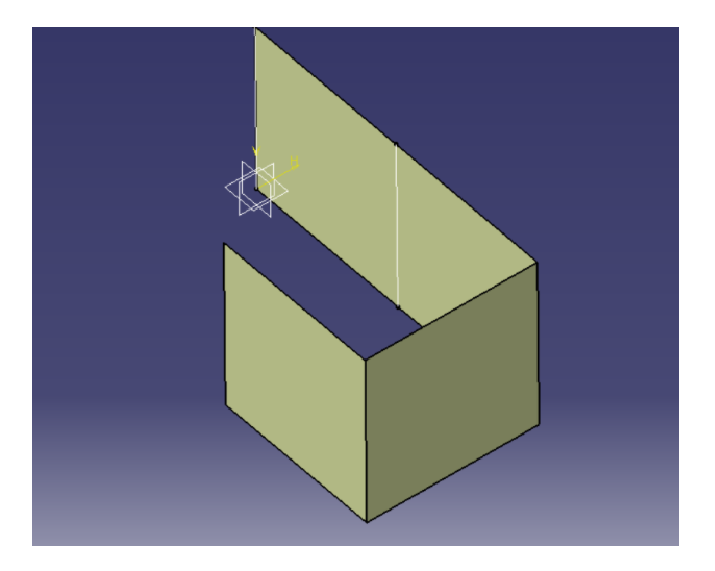
\includegraphics[keepaspectratio=true,scale=0.8]{figuras/estrutura14.eps}
 \caption{Segunda dobra}
 \label{estrutura14}
\end{figure}
\begin{figure}[H]
 \centering
   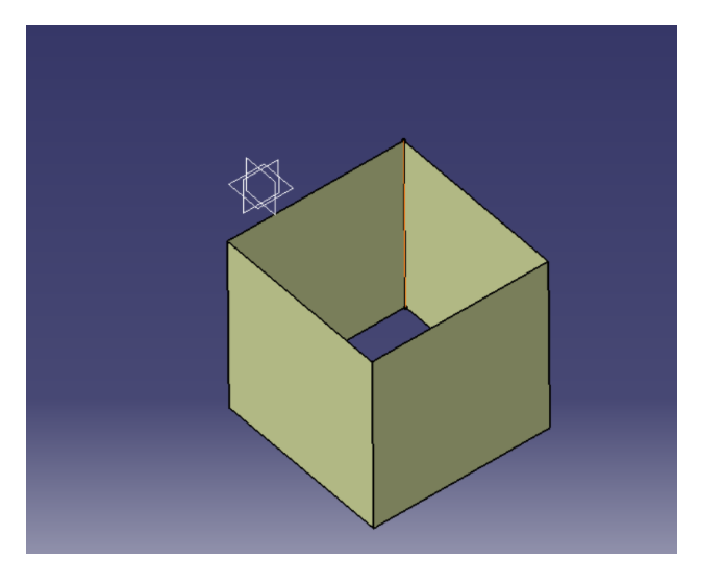
\includegraphics[keepaspectratio=true,scale=0.8]{figuras/estrutura15.eps}
 \caption{Última dobra}
 \label{estrutura15}
\end{figure}

Na junção entre as pontas da chapa foi pensado em uma junção por rebites ou por solda, porém sabemos que a solda em alumínio necessita de uma mão-de-obra especializada em solda TIG. Tendo isso em mente nossa primeira alternativa seriam os rebites. Porém sabemos que o compartimento estará no meio do lago e mesmo sem estar em contato direto com a água, é possível a infiltração de umidade  pelos rebites. Para corrigir esse problema temos a possibilidade de aplicar um produto impermeável nos furos como o silicone. Mais adiante falaremos sobre a solução para o isolamento térmico e essa solução pode resolver o problema dessa infiltração, como também o problema de sustentação falado anteriormente, porém caso isso não acontece já apresentamos soluções secundárias para cada problema isoladamente. Para a construção da tremonha foi pensado a mesma possibilidade, porém com dobras ânguladas. Como as dimensões das chapas são grandes não será possível utilizar a dobradora de chapas presente no galpão. Uma solução seria fazer a dobra comercialmente ou criar um mecanismo de dobra, a primeira opção num primeiro momento se mostra mais interessante para a integridade do projeto porém os custos terão que ser avaliados na hora da decisão.

\subsubsection{Conclusão acerca do Armazenador}

Com os cálculos e simulações realizadas foi possível estabelecer várias geometrias possíveis a partir do volume máximo necessário de  $1,232 m^3$. Utilizando chapas de 0.5 mm de alumínio foi possível suportar a carga sem haver deformação plástica do material, porém a necessidade de reforços para manter a geometria estável pode ser necessário. A princípio a geometria escolhida é um cubo de lados com 1,072 m de comprimento porém como sabemos o tamanho das chapas vendidas teremos que adaptar um pouco esse lado  mas a estrutura será muito próxima de um cubo ainda assim, essa geometria é de fácil fabricação e possui uma estabilidade maior que o cilindro se tratando de chapas de alumínio. Essa geometria suporta o esforço necessário para suportar a carga de ração e o próprio peso da estrutura. Na sua fabricação, usaremos a dobra de chapas e rebites para fixar a estrutura, esse processo pode ser terceirizado devido as limitações dos equipamentos disponíveis no galpão da FGA. Para impermeabilizar os furos dos rebites utilizaremos silicone, isso se a solução para isolamento térmico já não tratar disso.

\subsubsection{Isolamento Térmico}

O material isolante térmico tem a função de impedir a troca de calor do sistema com a vizinhança. A transferência de calor se manifesta na fronteira na forma de condução, convecção e ou radiação.

Os materiais porosos e fibrosos sao excelentes isolantes térmicos. Os espaços sem material sao preenchidos naturalmente por ar, com isso adquire maior conservação de energia, reduzindo a troca de calor, garante o controle da temperatura a fim de proteger o sistema, geralmente tem instalação rápida e barata e não é inflamável. Existem inúmeros materiais que oferecem um bom isolamento térmico, dependendo da temperatura do sistema e da vizinhança o material varia a espessura e consequentemente o valor para aquisição.

Será apresentado abaixo 3 opções como isolamento térmico

\subsubsubsection{Alumínio Corrugado}

\begin{figure}[H]
 \centering
   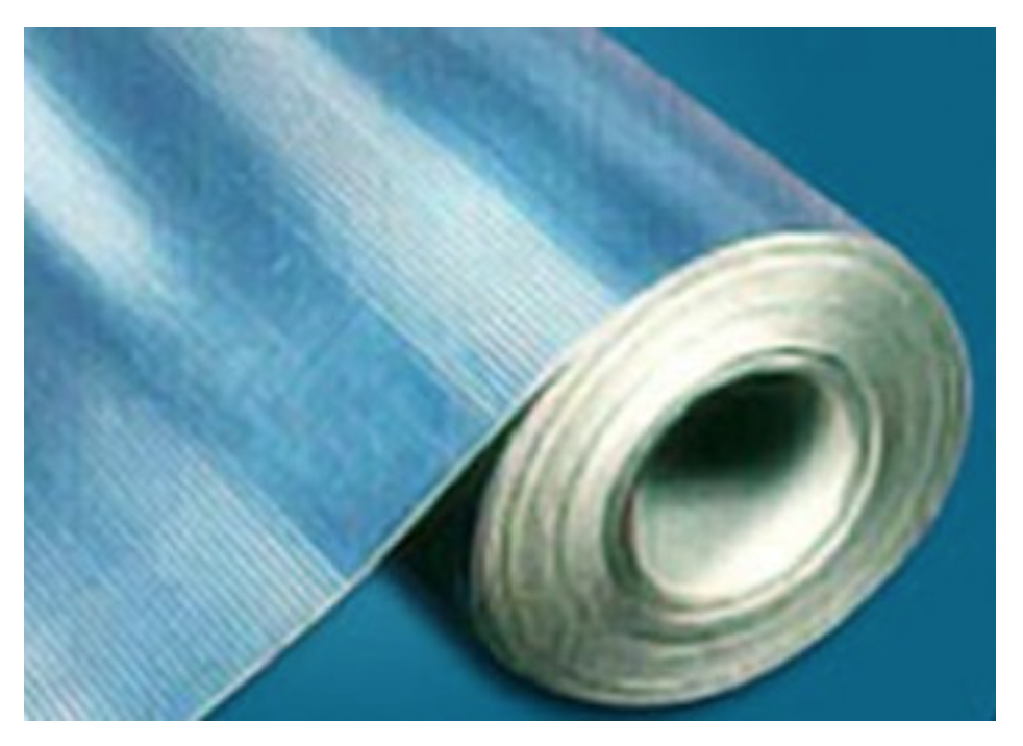
\includegraphics[keepaspectratio=true,scale=0.8]{figuras/aluminio.eps}
 \caption{Alumínio corrugado}
 \label{aluminio}
\end{figure}

O alumínio corrugado é uma opção nao muito interessante, pois a proposta principal dele é a proteção contra intempéries, não possui grande característica de isolar o sistema termicamente. Ele seria uma boa opção se o material escolhido para confecção do armazenador fosse o aço, mesmo assim teria q haver um outro material usado simultaneamente para adquirir um melhor isolamento térmico.\cite{isar}

PRINCIPAIS CARACTERÍSTICAS DO ALUMÍNIO CORRUGADO\cite{isar}:
\begin{itemize}
  \item Aplicação fácil e rápida;
  \item Pode ser reaproveitado;
  \item Remoção fácil e sem prejudicar a estrutura;
  \item Não é necessária pintura ou manutenção;
\end{itemize}

\subsubsubsection{Isoflex  Painel}

O Isoflex Painel é constituído de Poliuretano ,uma espuma rígida, predominantemente utilizada na técnica da isolação térmica.\cite{isar}

Baixo fator de condutividade térmica do painel de poliuretano, permite conseguir o dobro de eficiência térmica que se obteria com qualquer outro material isolante, fazendo com que seja necessário 50\% a menos de espessura em relação aos outros materiais. A baixa absorção de umidade o torna interessante pelo local que será implantado. Além disso a estrutura ganharia rigidez dimensional.\cite{isar}

A grande desvantagem desse sistema se resume a custos. Para utilizar essas placas como isolante deverá ser feita um “painel-sanduíche” com elas, sendo duas camadas de alumínio e esta camada de espuma de poliuretana no meio, assim dobrando os custos com a chapa de alumínio.\cite{isar}

\begin{figure}[H]
 \centering
   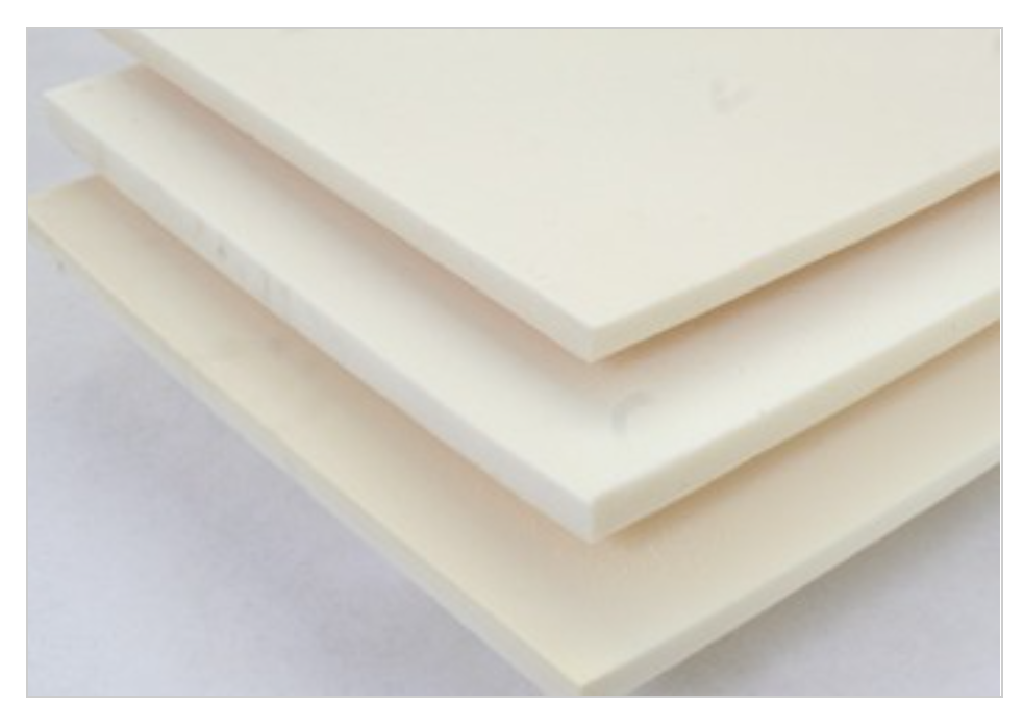
\includegraphics[keepaspectratio=true,scale=0.8]{figuras/isoflex.eps}
 \caption{Painel de isoflex}
 \label{isoflex}
\end{figure}

\begin{table}[]
\centering
\caption{Dados técnicos Isoflex}
\label{dadosisoflex}
\begin{tabular}{|l|l|l|l|}
\hline
Propriedades                       & Dimensão & $32/36 Kg/m^3$ & $36/40 kg/m^3$ \\ \hline
Cheiro                             & -        & Nenhum      & Nenhum      \\ \hline
Cor                                & -        & Amarela     & Amarela     \\ \hline
Resistência à compressão com       & $\frac{kg}{cm^2}$ & $1.5$         & $1.7$         \\ \hline
10\% de recalque.                  &          &             &             \\ \hline
Temperatura míxima que suporta     & 0{\degree}C      & -200        & -200        \\ \hline
Temperatura máxima que suporta     & 0{\degree}C      & 100         & 100         \\ \hline
Absorção de água após 24h submersa & Vol\%    & 1           & 1           \\ \hline
Ascenção Capilar                   & -        & Nenhuma     & Nenhuma     \\ \hline
Coef. condut. térmica              & Kcal     & 0,016       & 0,016       \\ \hline
Temperatura 10{\degree}C                   & m h{\degree}C    &             &             \\ \hline
Células fechadas                   & -        & Mínimo 90\% & Mínimo 85\% \\ \hline
Resist. aos Solventes              & -        & Excelente   & Excelente   \\ \hline
\end{tabular}
\end{table}

\subsubsubsection{Manta refletiva metalizada}

\begin{figure}[H]
 \centering
   \includegraphics[keepaspectratio=true,scale=0.8]{figuras/manta.eps}
 \caption{Manta refletiva metalizada}
 \label{manta}
\end{figure}

Segundo a fabricante Coberfoil, este bloqueio térmico é chamado de subcoberturas. Estas sim, mantas de isolamento térmico e hídrico, são refletivas e de alta performance. Desenvolvidas pela NASA nos anos 50 tiveram a parte de metalizado tratado e polido substituídas gradativamente por filme de polipropileno metalizado, com mesmo efeito, sem causar dano ao ambiente.\cite{Coberfoil}
Segundo a fabricante Coberfoil, as Mantas Refletivas Coberfoil® são bastante resistentes e não se deterioram. Usadas sob as telhas; interceptam de 90 a 95\% de calor na dupla face, 70 a 75\% de calor na monoface, segundo o Instituto de Pesquisas Tecnológicas – IPT. Também são capazes de reduzir em até 10{\degree}C a temperatura interna.\cite{Coberfoil}

A empresa não fornece o coeficiente de condutividade térmica, tornando-o assim de difícil comparação. Porém tomando os dados fornecidos pela empresa como verdadeiros, esta opção se torna bastante interessante para a aplicação desejada no projeto.

\subsection{Sustentação e Estabilidade}

O projeto estrutural do Alimentador deve levar em consideração alguns fatores importantes para que haja sucesso na solução encontrada; alguns princípios aerodinâmicos, estruturais, hidrodinâmicos devem ser considerados para a apropriada modelagem do problema. Além de fatores de solução e integração mecânica entre sistemas para que o conjunto funcione integralmente sem interferências e má conexão entre os elementos que o compõem.

Das considerações de sustentação hidrostática, deve-se observar os princípios de empuxo e estabilidade \cite{Frank} descobertos por Arquimedes e onde atua a força de empuxo, no centro de massa ( considerando densidade uniforme). Esse ponto é chamado centro de empuxo, usualmente indicado por CE.

\begin{figure}[H]
 \centering
   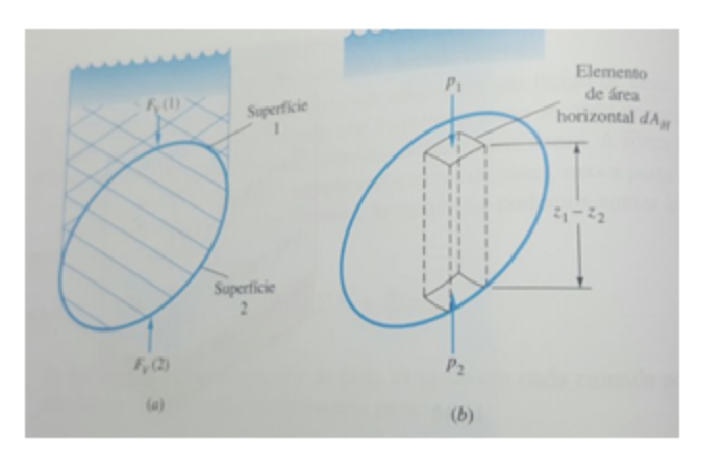
\includegraphics[keepaspectratio=true,scale=0.8]{figuras/circulos_1.eps}
 \caption{Estabilidade da estrutura flutuante 1}
 \label{estabilidade1}
\end{figure}

\[Fe = Fv_{2} -Fv_{1}\]
\[Fe = (PesoDoFluidoAcimaDe2) - (PesoDoFluidoAcimaDe1)\]
\[Fe = PesoDoFluidoEquivalenteAo Corpo\]

Em relação à estabilidade do sistema flutuante, deve-se observar os critérios de estabilidade (páginas 104 e 105 da referência \cite{Frank})

\begin{figure}[H]
 \centering
   \includegraphics[keepaspectratio=true,scale=0.8]{figuras/circulos_2.eps}
 \caption{Estabilidade da estrutura flutuante 2}
 \label{estabilidade2}
\end{figure}

O cálculo da estabilidade se dá através de informações geométricas do volume submerso de sustentação e da distância do metacentro ao CG que deve ser positiva, ou seja, o metacentro deve estar acima do CG, desde que o centro de empuxo esteja abaixo do nível da água. Caso o centro de empuxo esteja acima da CG, o corpo se encontra necessariamente em estabilidade.

\[\overline{MG} = \frac{I_{0}}{Vsubmerso} - \overline{GE}\]

Condição de estabilidade $\overline{MG} > 0$, quanto maior, mais estável será o objeto flutuante.
Realizando os cálculos com base de 2x2 devido as dimensões dos menores tanques de 3x3 e profundidade de 0,2m; de forma que os Alimentadores possam ficar lado a lado em uma sequencia de tanques sem que haja colisão entre as estruturas.

\[I_{0} = \frac{200.200^3}{12} = 133.10^6 ;Vsubmerso = 0,2.2.2 = 0.8[m^3] = 8.10^5[mm^3]\]

Estimando a distância do CG da estrutura e a superfície da água em $0,8m^3$, temos que:

\[\overline{MG} = \frac{133.10^6}{8.10^{^-5}} - 80=166,25 -80 =86,25\]

Segundo a literatura \cite{Frank} haverá estabilidade estática da estrutura; embora ainda iremos buscar parâmetros e referências para o PC2.

Além dos critérios de estabilidade relacionados à sustentação hidroestática, deve-se observar o arrasto devido ao escoamento em rajadas de vento, que podem ou não ser relevantes na dinâmica do sistema flutuante tanto para a estabilidade do sistema, quanto para o dimensionamento dos fixadores do Alimentador aos tanques.

O arrasto possui duas componentes que exercem influência e são objetos de estudo e aplicados em projetos aeroespaciais ou aeronáuticos.

As componentes do arrasto, são a de pressão e a de atrito de superfície respectivamente. Para esta aplicação, iremos considerar o escoamento incompressível (Mach < 0.3), invíscido em Placa Plana sem forças de campo atuantes.

Desconsiderar o arrasto devido ao atrito de superfície também é coerente, devido ao fato de que sua parcela representa muito pouco em relação ao arrasto devido a pressão do escoamento perpendicular à área do corpo.

Considerando \textbf{Cd = 2} ( Coeficiente de arrasto ) - Placa Plana, devido a geometria da superficie perpendicular de maior area:

\[Fa\frac{[kg.m]}{s^2} = \frac{1}{2}{c_{d}}\rho\frac{^[kg]}{[m^3]}A[m^2][V^2\frac{[m^2]}{[s^2]}]\]

Segundo referências pesquisadas até junho de 2017 \cite{tempo},\cite{globo} e \cite{vento}  foi possível observar que há medias de velocidade do vento que giram em torno de \textbf{10km/h} com rajadas de \textbf{20km/h} em dias normais na região de Palmas - TO, sendo que nessa região os registros mais elevados estão em torno de \textbf{80km/h}. Em pesquisa realizada sobre rajadas de vento recorde no Brasil, \textbf{145km/h} foi uma das maiores registradas em Santa Maria - RS.

Segundo o projeto preliminar do armazenador, a área de seção lateral é de $1m^2$ no caso de escoamento perpendicular a face quadrada ( Placa Plana ) e $1,41m^2$ no caso de escoamento perpendicular ao armazenador como perfil triangular. Como a parcela mais relevante ao arrasto nesses casos é a parcela ao arrasto por pressão e o cd da placa plana é o maior de todos, iremos considerar o pior caso, no caso placa plana de As = $1m^2$,  Cd = 2 e $\rho = 1,23 [\frac{kg}{m^3}]$

\[Fs_{rc} = \frac{1}{2}.2.1,23 \frac{[kg]}{[m^3]}.(40,28^2)\frac{[m^2]}{[s^2]} .1[m^2] = 1995,6[N]\]
\[Fr_{c} = \frac{1}{2}.2.1,23 \frac{[kg]}{[m^3]}.(22,22^2)\frac{[m^2]}{[s^2]} .1[m^2] = 607,3[N]\]
\[Fr_{m} = \frac{1}{2}.2.1,23 \frac{[kg]}{[m^3]}.(11,11^2)\frac{[m^2]}{[s^2]} .1[m^2] = 151,82[N]\]

A estabilidade será projetada a partir desses dados e de acordo com a relação entre viabilidade de projeto e segurança, ou seja, tentar-se-á obter estabilidade para as maiores rajadas já registradas, embora, caso isto aumente consideravelmente os custos do projeto ou a dificuldade de integração com outras áreas, esse fator possa ser considerado para rajadas médias de determinadas regiões no Brasil.

Para o cálculo do volume de sustentação deve-se substituir os valores de massa específica do material que será utilizado para dar sustentação à estrutura, este deve ser menos denso do que a água.

$ Msist[kg] = \rho\frac{[kg]}{[m^3]}; Fe = \rho_{fluidodeslocado}[\frac{kg}{m^3}] g[\frac{m}{s^2}]V[m^3]$

\[Fe = Fn = Vsust[m^3] = \frac{Msist[kg].g\frac{[m]}{[s^2]}}{\rho\frac{[kg]]}{[m^3]}.g\frac{[m]}{[s^2]}} =\frac{Msist[kg]}{\rho\frac{[kg]]}{[m^3]}}  = \frac{400[kg]}{970\frac{[kg]]}{[m^3]}} = 0,4123[m^3]\]

Esses valores nos permitem observar e garantir que o projeto seja viável para darmos prosseguimento em considerações mais refinadas para modelagem da estrutura.

Devido ao volume de sustentação preliminar para a massa estimada para todo o sistema ser relativamente pequeno, e a possibilidade e necessidade de se utilizar recipientes com formato fixado e determinado pelo mercado, atrelado ao fato de haver maior carga durante os momentos de recarga do armazenador, acrescentar-se-á a parcela de carga relativa a um perfil ergonômico 95\% segundo a tabela antropométrica  brasileira, que é de 85kg, para efeitos de cálculo e atender casos de trabalhadores fora da média, excederemos o percentil 95\% em 15kg, 17\% , além da massa de um saco de ração de 25kg

\[Fe = Fn = Vsust[m^3] = \frac{525[kg]]}{970[kg/m^3]} = 0,5412 [m^3]\]

E por fim, após decidir o recipiente utilizado para gerar o volume de sustentação calcularemos a sustentação total da solução de projeto.

Há possibilidade de reutilizar recipientes de material plástico (PET, os quais são abundantes e descartados ou comercializados localmente em várias regiões de relativa baixa ou alta atividade industrial.

\begin{figure}[H]
 \centering
   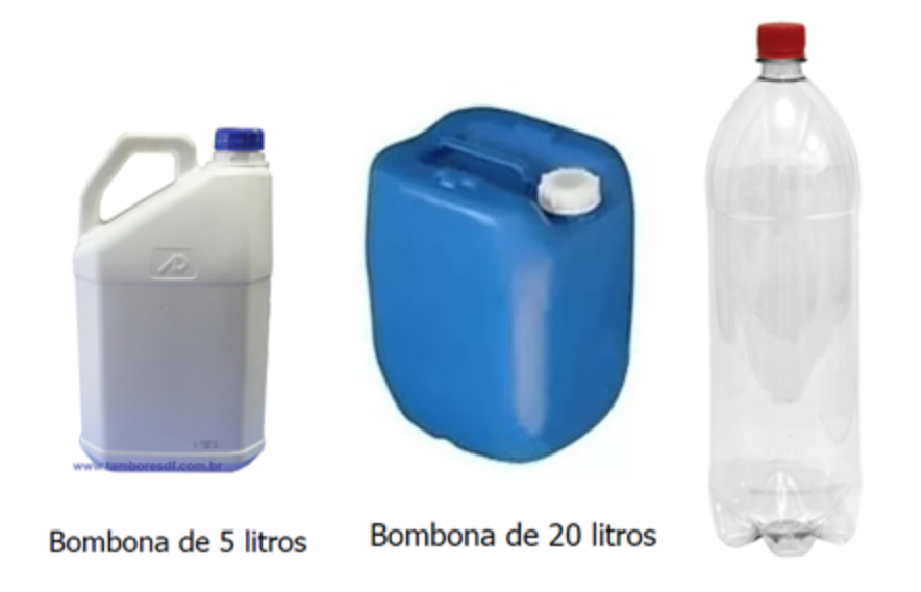
\includegraphics[keepaspectratio=true,scale=0.8]{figuras/garrafas.eps}
 \caption{Pets para a criação da boia 1}
 \label{pets0}
\end{figure}

\begin{figure}[H]
 \centering
   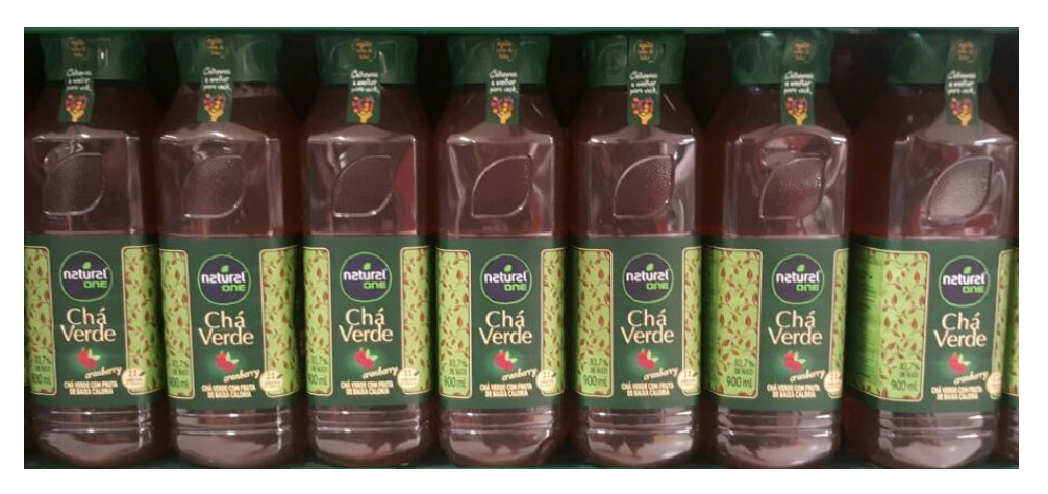
\includegraphics[keepaspectratio=true,scale=0.8]{figuras/garrafa_1.eps}
 \caption{Pets para a criação da boia 2}
 \label{pets1}
\end{figure}

\begin{figure}[H]
 \centering
   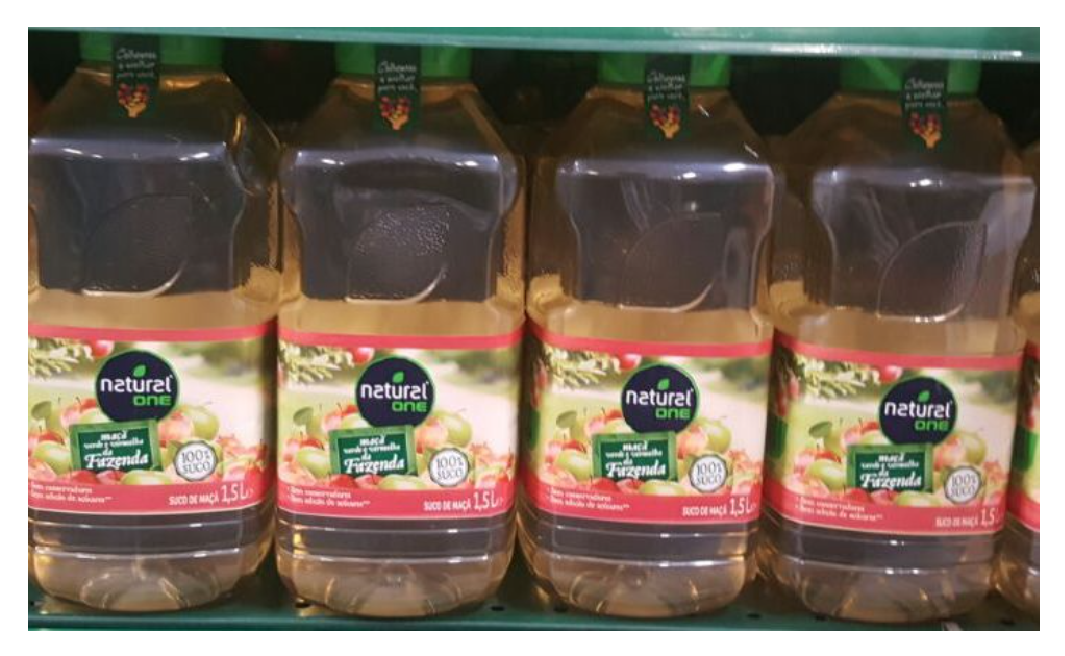
\includegraphics[keepaspectratio=true,scale=0.8]{figuras/garrafa_2.eps}
 \caption{Pets para a criação da boia 3}
 \label{pets2}
\end{figure}

Também existe a possibilidade de utilizar boias comerciais \cite{nauticexpo}  ou decks \cite{smartpier} para sustentação.

\begin{figure}[H]
 \centering
   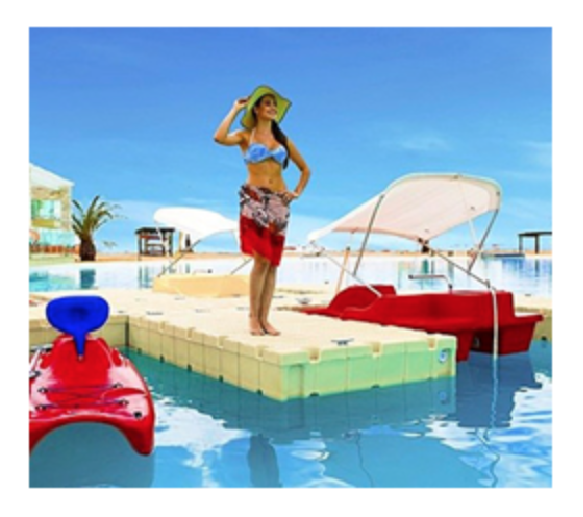
\includegraphics[keepaspectratio=true,scale=0.8]{figuras/boias.eps}
 \caption{Boias comerciais}
 \label{Boias_cormercias}
\end{figure}

Em relação à sustentação, a escolha será feita a partir do melhor custo benefício e otimização de espaço dentro da estrutura de sustentação, já que os recipientes serão utilizados para armazenar o ar o qual gera sustentação para a estrutura; e serão organizados em pacotes.

A matriz de decisão, presense na tabela \ref{matriz_sustetacao} dos recipientes de sustentação possuem os seguintes pesos de importância para cada parâmetro: Custo = 4; Acessibilidade = 2; Segurança = 5; Eficiência de Empacotamento = 4.

\begin{sidewaystable}
  \begin{table}[H]
  \centering
  \caption{Matriz de decisão dos recipientes de sustetação}
  \label{matriz_sustetacao}
  \begin{tabular}{|l|l|l|l|l|l|}
  Tipo                        & Custo & Acessibilidade & Segurança (Redundância) & Eficięncia de Empacotamento & Total \\ \hline
  Garrafas PET (Refrigerante) & 2     & 2              & 2                       & 1                           & 5,5   \\ \hline
  Garrafas PET (Suco)         & 1     & 2              & 2                       & 2                           & 6,5   \\ \hline
  Bombonas 20l                & 1     & 2              & 1                       & 2                           & 5,25  \\ \hline
  Bombonas 5l                 & 1     & 2              & 2                       & 1                           & 5,5   \\ \hline
  Bóias Comerciais            & 0     & 1              & 2                       & 1                           & 4     \\ \hline
  Deck Comercial              & 0     & 1              & 2                       & 2                           & 5     \\ \hline
  Camaras de Ar               & 2     & 2              & 1                       & 2                           & 6,25 \\ \hline
  \end{tabular}
  \end{table}
\end{sidewaystable}
A princípio haverá a escolha entre os pets de suco e a confecção de câmaras de ar, dependendo dos custos e acessibilidade de cada um, após a escolha definitiva será projetado o sistema estrutural que armazenará esses pacotes de sustentação.

\subsection{Sistema de Alimentação}

\subsubsection{Dimensionamento}

O sistema de alimentação do alimentador baseado na estrutura já decidida do armazenador. A solução pensada, foi utilizar uma rosca transportadora. A rosca transportadora é uma rosca helicoidal sem fim que faz o transporte horizontal de grãos em geral a partir de um armazenador.

Se trata de um equipamento muito simples e muito utilizado para fazer o transporte de grãos. Consiste em uma rosca helicoidal acomodada dentro de um tubo ou calha, ao qual aplica-se uma rotação a partir de um motor \cite{ss}. Para utilizar esse sistema e garantir que a dose certa de ração seja dada o grupo optou por utilizar uma câmara de dispersão. Essa câmara servirá para receber a ração e por intermédio de células de cargas (sensores) medir se a dose de ração está correta. Após isso o motor será desligado e a ração será despejada de uma vez para o tanque. O sistema de ativação do despejo poderá ser mecânico através de molas ou por atuador eletrônico, sendo que a decisão dependerá de testes futuros sobre a estrutura.

\begin{figure}[H]
 \centering
   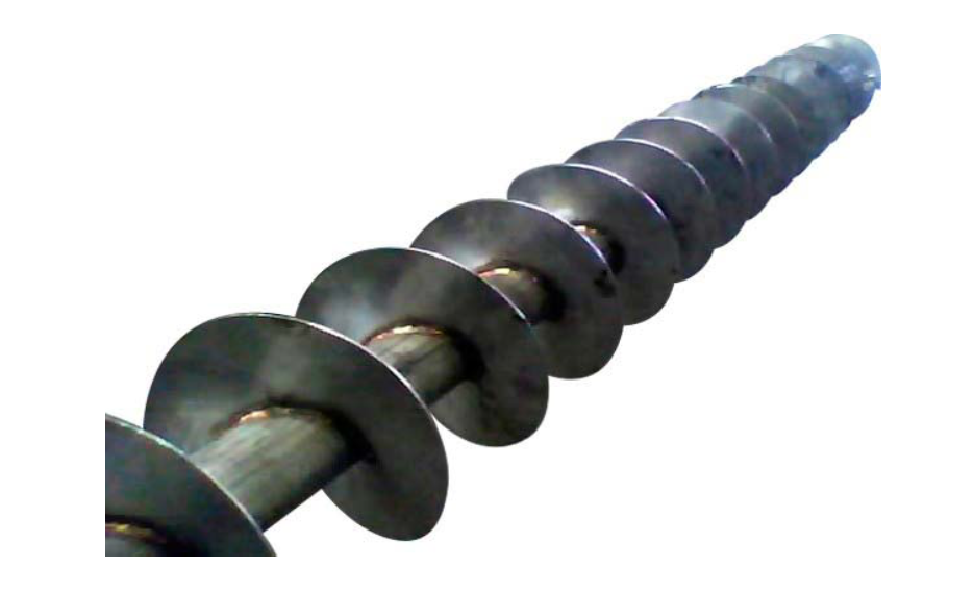
\includegraphics[keepaspectratio=true,scale=0.8]{figuras/rosca.eps}
 \caption{Rosca helicoidal}
 \label{rosca}
\end{figure}

Para utilização desse sistema devemos estimar a vazão Q, a potência P e o torque T para a escolha do motor que fará a movimentação desse eixo, onde parâmetros geométricos como o diâmetro maior e menor são necessários. A princípio o grupo comprará a rosca e fará uma adaptação para encaixar no motor escolhido. Uma possível alternativa de compra de rosca tem as seguintes dimensões:

\begin{itemize}
  \item Diâmetro do helicóide = 55mm
  \item Diâmetro do eixo = 15mm
  \item Passo = 44mm
  \item Comprimento = 11 cm
\end{itemize}

\begin{figure}[H]
 \centering
   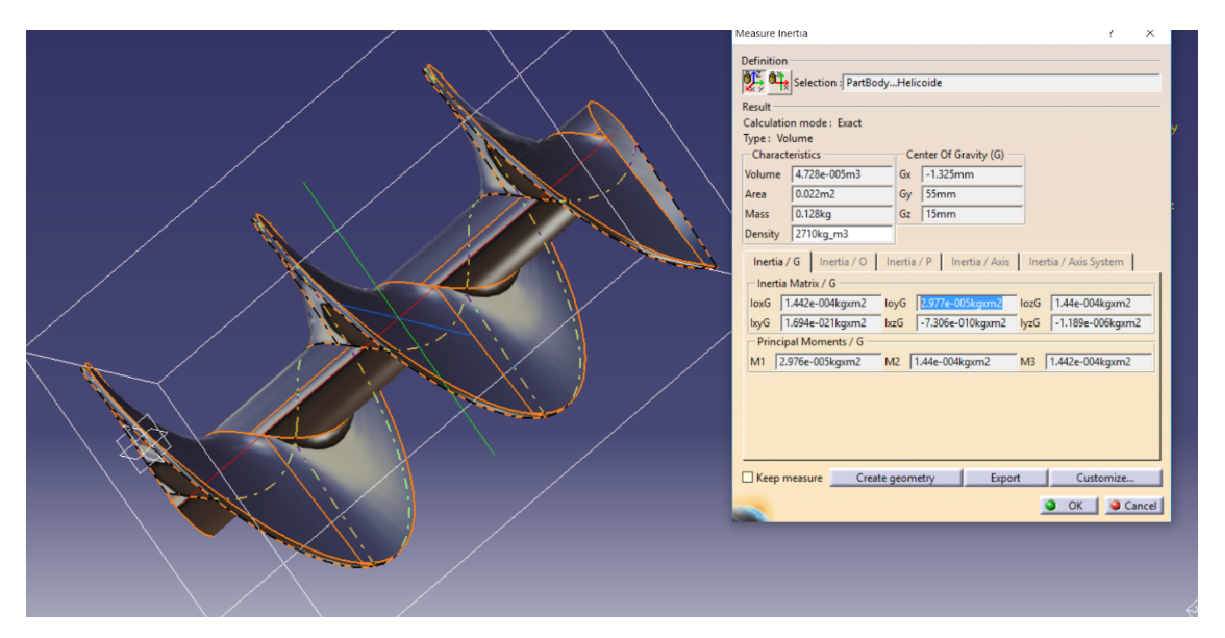
\includegraphics[keepaspectratio=true,scale=0.8]{figuras/rosca_cad.eps}
 \caption{Helicoide}
 \label{rosca_cad}
\end{figure}

Modelando a rosca em CAD com material de alumínio encontramos uma massa de 128 g e um momento de inércia  (Io) de $2,977x10^-5 kg*m^2$. Esses dados foram usados para verificar a potência necessário do motor. Para acomodar o motor e o helicóide é necessário um estrutura acoplada ao armazenador e à câmara de dispersão, a seguir apresentaremos um primeiro esboço dessa estrutura.

\begin{figure}[H]
 \centering
   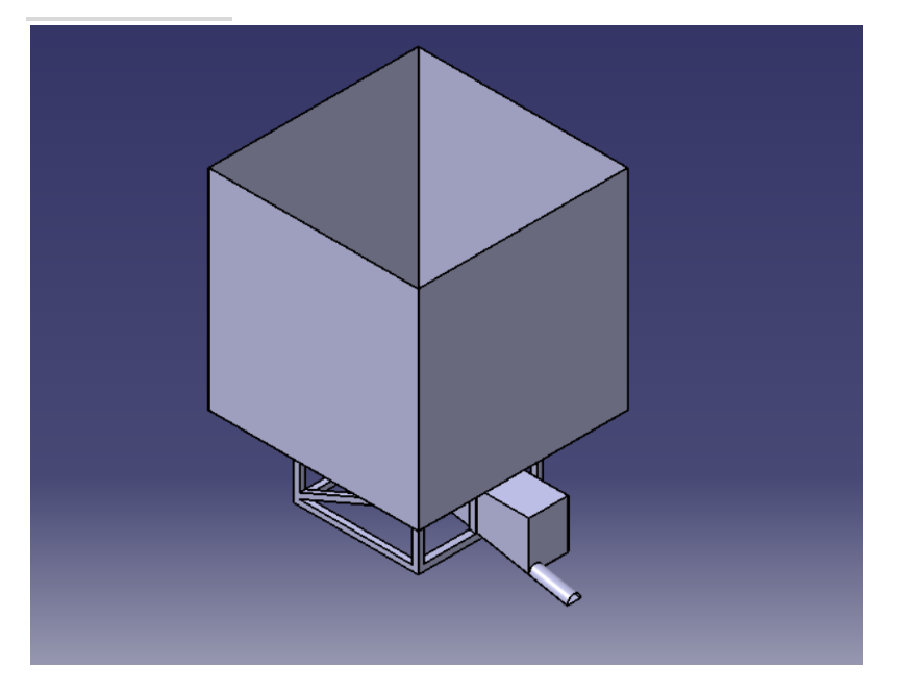
\includegraphics[keepaspectratio=true,scale=0.8]{figuras/vista_iso_alimentador.eps}
 \caption{Vista isométrica do Alimentador}
 \label{vista_iso_alimentador}
\end{figure}

\begin{figure}[H]
 \centering
   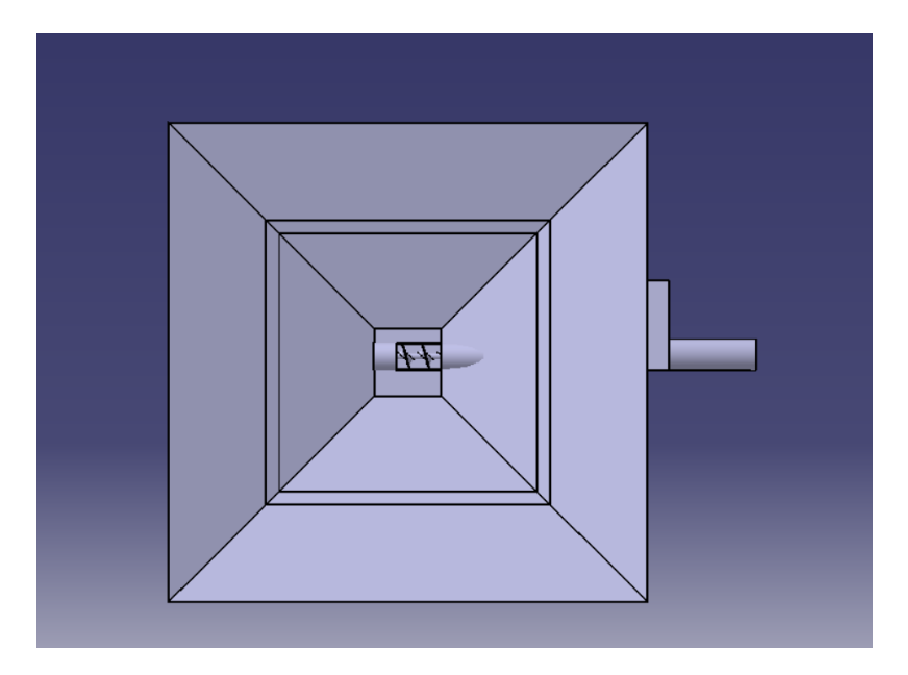
\includegraphics[keepaspectratio=true,scale=0.8]{figuras/vista_superior.eps}
 \caption{Vista superior do Alimentador}
 \label{vista_superior}
\end{figure}

\begin{figure}[H]
 \centering
   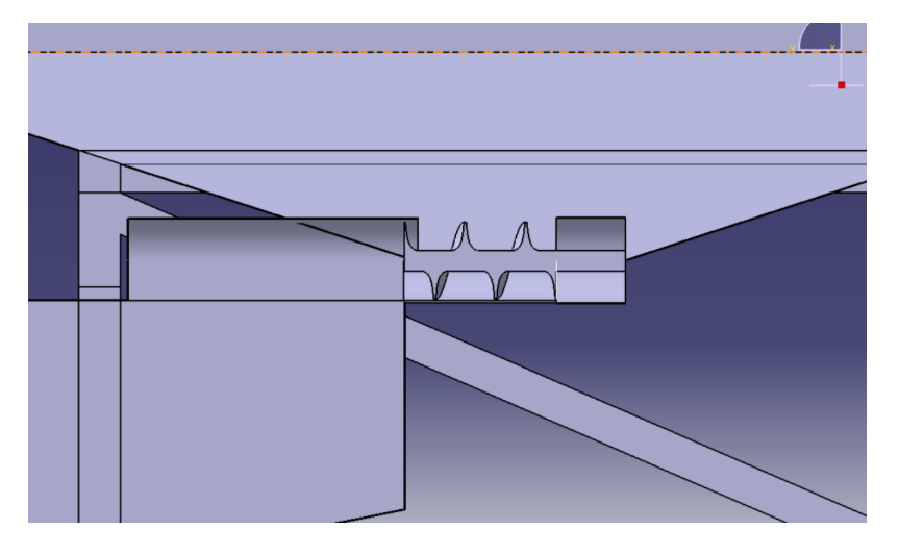
\includegraphics[keepaspectratio=true,scale=0.8]{figuras/corte_lateral.eps}
 \caption{Vista em corte lateral do alimentador}
 \label{corte_lateral}
\end{figure}

\begin{figure}[H]
 \centering
   \includegraphics[keepaspectratio=true,scale=0.8]{figuras/corte_camara.eps}
 \caption{Câmara de dispersão}
 \label{corte_camara}
\end{figure}

Para calcular o volume necessário da câmara foi utilizada uma dose de ração de aproximadamente 4,5 kg. E utilizamos uma geometria trapezoidal para aproveitar a aceleração da gravidade na dispersão da ração. O volume foi calculado estimando valores e utilizando uma planilha no excel para estimar os cálculos. Para fazer a dosagem da ração utilizaremos células de carga, que são sensores de força. Há a possibilidade ser utilizados mais de um sensor para fazer a medição, e para utilizar esse sensor pode ser necessária a utilização de uma chapa “solta” no fundo da câmara de dispersão para servir como balança, como não há experiência do grupo com o uso deste sensor serão feitos testes para avaliar a melhor forma de posicionamento do mesmo.

\begin{figure}[H]
 \centering
   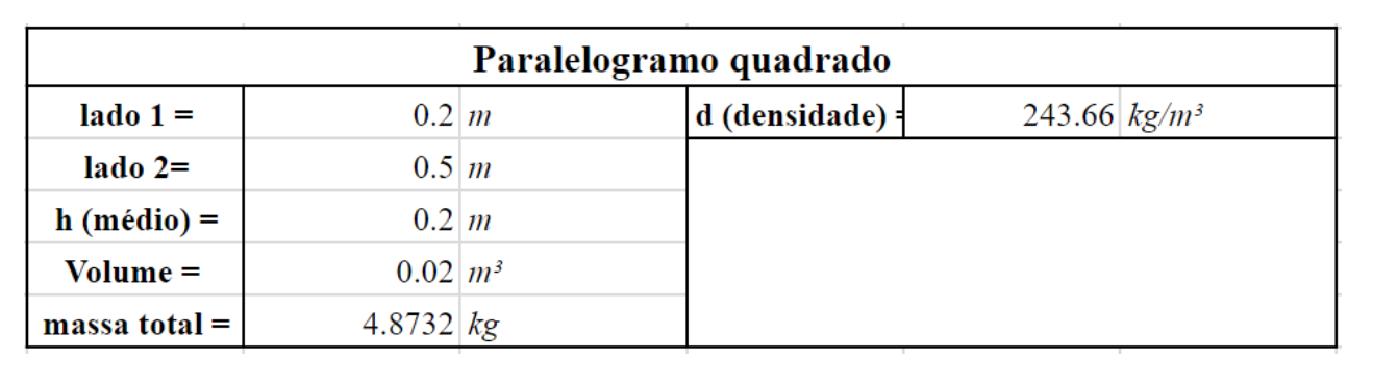
\includegraphics[keepaspectratio=true,scale=0.8]{figuras/quadro_parelolo.eps}
 \caption{Cálculo do volume da câmara de dispersão}
 \label{quadro_parelolo}
\end{figure}

\subsubsection{Processos de fabricação}

Para a fabricação do sistema de alimentação podemos dividi-lo em 2 partes: a câmara de dispersão e a câmara de transporte. A câmara de transporte consiste na estrutura que fará o transporte da ração do armazenador até a câmara de dispersão.

\begin{figure}[H]
 \centering
   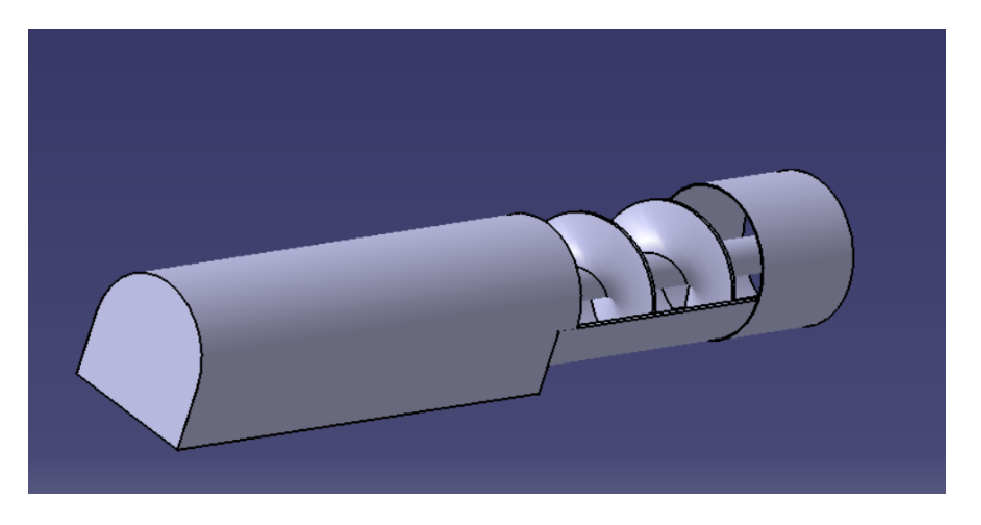
\includegraphics[keepaspectratio=true,scale=0.8]{figuras/camara_transporte.eps}
 \caption{Câmara de transporte}
 \label{camara_transporte}
\end{figure}

O CAD acima pode ser simplificado em um tubo cortado que passará por dentro da tremonha do armazenador e acomodará a rosca transportadora e o motor. No caso estamos utilizando uma rosca de 11 cm de comprimento, porém esse comprimento não está fixo e dependerá de uma análise mais específica tanto da eficácia do sistema quanto dos custos, podendo ser utilizada uma rosca maior em torno de 1 m de comprimento. O tubo poderá ser de alumínio ou um tubo PVC que é facilmente encontrado comercialmente e revestido com chapas de alumínio se houver uma necessidade de robustez maior. Quanto à rosca existe a possibilidade de fabricação caso haja a necessidade de fabricar algo específico ou as outras soluções se mostrem com  um custo muito elevado sendo essa a última opção. A fabricação envolveria um eixo de aço (maciço ou tubo) e o helicóide formado por uma chapa fina de aço cortada nos moldes de necessários. Esse molde pode ser calculado de acordo com a figura a seguir.

\begin{figure}[H]
 \centering
   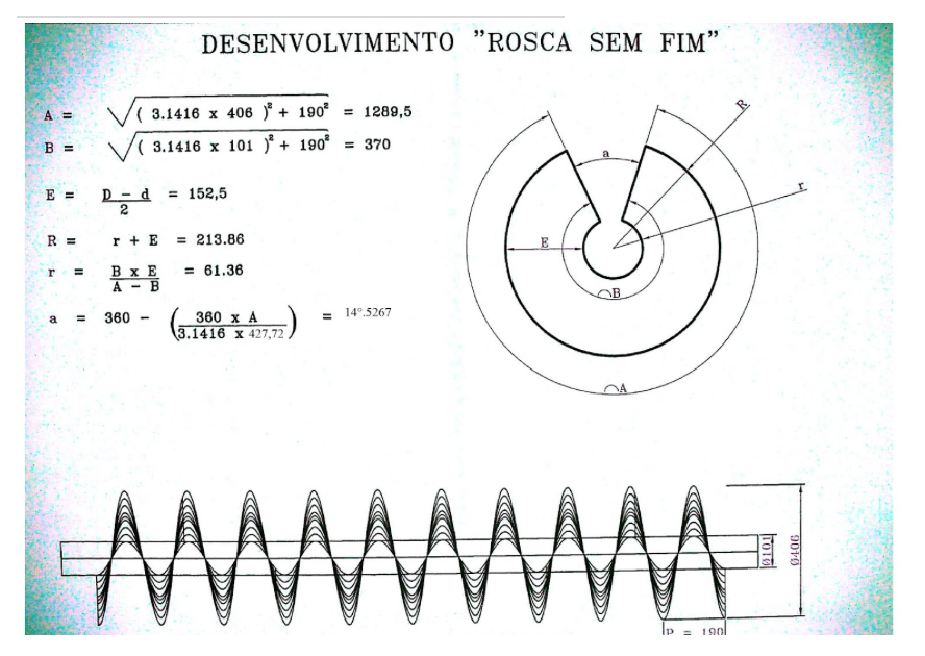
\includegraphics[keepaspectratio=true,scale=0.8]{figuras/calculo_de_roca.eps}
 \caption{Cálculo de rosca transportadora.}
 \label{calculo_rosca}
\end{figure}

Já a câmara de dispersão será produzida da mesma forma que o armazenador tendo como material as chapas de alumínio de 0,5mm, porém como suas dimensões são menores será possível utilizar a dobradora de chapas presente no Galpão da FGA se a mesma estiver disponível. A junção poderá ser pod rebites ou por solda, porém arrebitar se mostra a medida mais plausível, impermeabilizando os furos com silicone ou outra substância impermeabilizadora. Essa parte da estrutura ficará fixada na base do armazenador a princípio para que ambos se movam juntos não trazendo problemas ao sistema de alimentação. A junção entre as parte será feita por encaixe mecânico podendo o mesmo se dar por interferência ou folga, com um sistema misto de tolerância dimensional, ou se utilizando de travas mecânicas como entalhes e chavetas.

\subsubsection{Conclusão acerca do sistema de alimentação}

O sistema de alimentação é o subsistema estrutural responsável pela dosagem da alimentação e seu transporte do armazenador ao tanque. Ele utilizará um sistema de rosca transportadora que é muito difundido no transporte de grãos em várias áreas agrícolas e de alimentação de animais. Esse sistema conta com 2 (duas) partes principais: câmara de transporte e câmara de dispersão. Na câmara de transporte ficará acomodada a rosca transportadora e o motor e ela fará a conexão entre o armazenador e a câmara de dispersão. A câmara de transporte será feita em formato tubular, sendo a primeira opção um tubo PVC com possível reforço em alumínio, e uma segunda opção seria o tubo de alumínio. Já a câmara de dispersão terá uma capacidade inicial de armazenar até 4,87 kg, para isso uma estrutura feita em chapa de alumínio assim como o armazenador é a solução primária. A acomodação de um ou mais sensores de força é algo que necessita de uma avaliação posterior de posicionamento estrutural, mas seu uso é necessário para calcular a dose de ração. Para escoar a ração até o tanque será usado um atuador para abrir a porta que faz a ligação entre a estrutura e o tubo de alimentação, esse atuador poderá ser tanto eletrônico quanto mecânico.

\subsection{Custos do projeto estrutural}

Abaixo tem-se uma prévia dos custos que teremos na área estrutural

\begin{table}[H]
\centering
\caption{Tabela de custo do projeto estrutural}
\label{custo_estrutural}
\begin{tabular}{|l|l|l|l|l|}
\hline
MATERIAL                    & QUANTIDADE & VALOR R\$ & UNIDADE & VALOR TOTAL \\ \hline
Chapa de alumínio 5mm       & $mˆ2$        & 32        & 6 & 192       \\ \hline
Cantoneira de aluminio 5 cm & 6 mt       & 138       & 2   & 276    \\ \hline
Isolamento térmico          & $50 m^2$      & 165       & 1  & 165      \\ \hline
Rosca de transporte         & 11cm       & 55        & 1    & 55   \\ \hline
Bombonas                    & 20l        & 33        & 0    & 0   \\ \hline
Bombonas                    & 200l       & 3         & 200   & 600  \\ \hline
Total                       &         &           &        & 1288 \\ \hline
\end{tabular}
\end{table}

\subsection{Integração}

\subsubsection{Subsistemas internos}

Uma preocupação é que a montagem do sistema seja modular e que caso um subsistema falhe seja possível trocá-lo sem que o alimentador por inteiro fique inviabilizado. Para isso evitaremos o uso de solda e rebites nas junções entre eles, e substituiremos por encaixes dimensionais (interferência, justo ou folga), travas como chavetas e cupilhas ou a utilização de parafusos.

\subsubsection{Outros sistemas}

Se tratando dos outros sistemas do projeto a estrutura deve atender às demandas de cada área. Fazendo a acomodação de equipamentos específicos com demandas específicas. Já foi mencionado a acomodação do motor, porém sensores e componentes eletrônicos também terão que ser acomodados e necessitam ficar blindados para não correrem risco de danos. Essa acomodação será feita ponto a ponto, podendo necessitar de uma estrutura mais robusta ou apenas uma forma de fixação como cola, isolamento de cabos, entre outros. Essa especificação necessitará de uma definição geral acerca do projeto e por isso não é possível determinar cada estrutura utilizada neste momento.

\subsubsection{Protótipo em CAD}

Para finalizar apresentamos o protótipo do projeto em CAD.

\begin{figure}[H]
 \centering
   \includegraphics[keepaspectratio=true,scale=0.8]{figuras/prototipo.eps}
 \caption{Protótipo em CAD do Alimentador}
 \label{prototipo}
\end{figure}
